% !TEX program = arara
% arara: pdflatex
% arara: biber
% arara: pdflatex
% arara: pdflatex
% arara: clean: { files: [ Paper.out ] }
% arara: clean: { files: [ Paper.aux, Paper.bbl ] }
% arara: clean: { files: [ Paper.bcf, Paper.blg ] }
% arara: clean: { files: [ Paper.log, Paper.run.xml ] }
% arara: clean: { files: [ Paper.toc, Paper-blx.bib ] }
% 

\documentclass{Paper}
\usepackage{ngerman}
\usepackage[utf8]{inputenc}
\usepackage{todonotes}
\usepackage{tikz}
\usepackage{pgf-pie}
\usepackage{pgfplots}

\begin{document}

\maketitle

% % % % %

\tableofcontents
\clearpage
	
\section{Abstrakt}
\todo{Autor: Berna}
	Yo
	
\section{Einleitung}
\todo{Autor: Kim}
	Yo
	
\section{Methode}
\todo{Autor: Nizan \& Alina (\& Marvin \& Daniel)}
	Yo
	
\section{Ergebnisse}
\todo{Autor: Jana \& Chovi (\& Nicole \& Svenja)}

kleines test pie chart mit richtigen zahlen



- ,,Hatten Sie Spaß?'' $<=>$ Zeitwahrnehmung  ? 
\begin{figure}[ht]
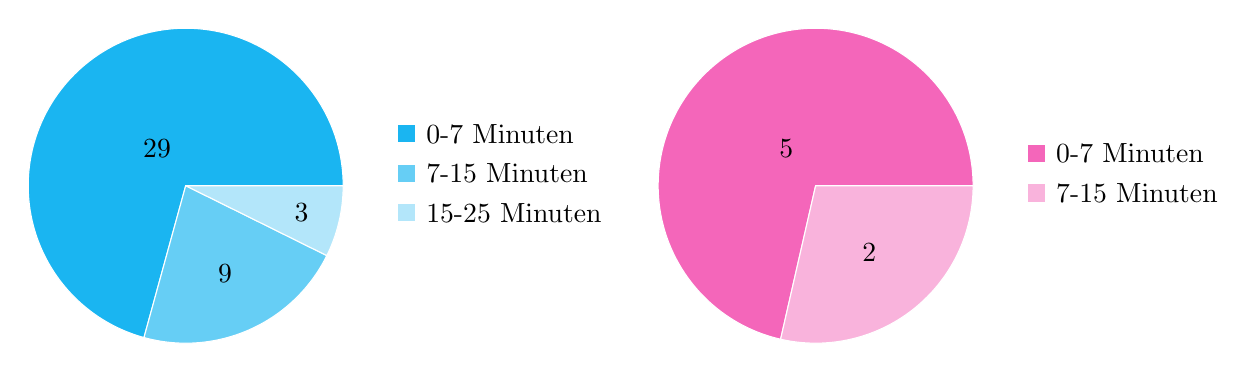
\begin{tikzpicture}
\tikzset{lines/.style={draw=white},}
\pie[color={cyan!90, cyan!60, cyan!30},radius = 2 ,sum=auto, after number=,text=legend,every only number node/.style={text=black},style={lines}]{29/0-7 Minuten,9/7-15 Minuten,3/15-25 Minuten}


\tikzset{lines/.style={draw=white},}
\pie[pos={8,0},radius = 2, color={magenta!60, magenta!30},sum=auto, after number=,text=legend,every only number node/.style={text=black},style={lines}]{5/0-7 Minuten,2/7-15 Minuten}
\end{tikzpicture}
\caption{Links: hatten Spaß. Rechts: hatten \textit{keinen} Spaß}
\end{figure}

	
- Szenarien sortieren kurz $->$ lang

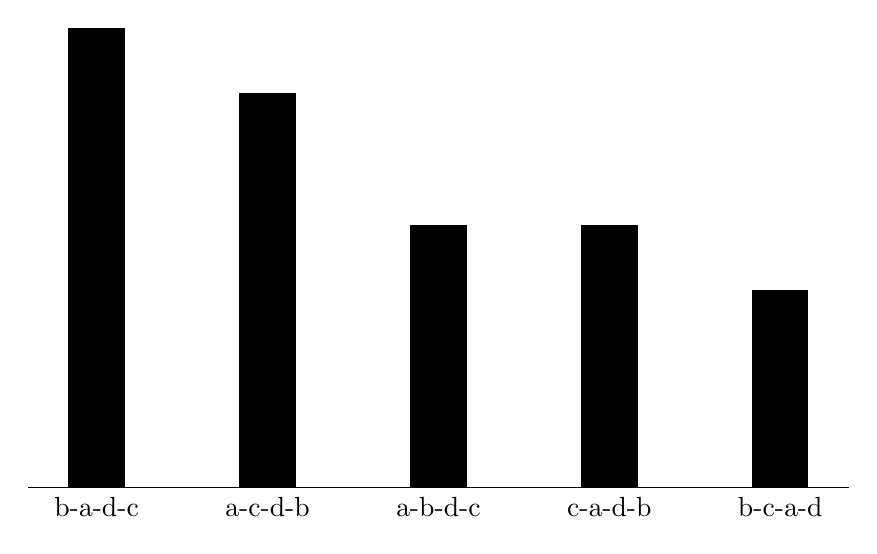
\begin{tikzpicture}
\begin{axis}[
     width  = 12cm,
     hide y axis,
     axis x line*=bottom,
     height = 8cm,
    bar width=20pt,
     symbolic x coords={b-a-d-c, a-c-d-b, a-b-d-c, c-a-d-b, b-c-a-d},
     %nodes near coords,
     ymin=0,
     xtick=data
     ]
     
     
     \addplot[ybar, fill=black] coordinates {
          (b-a-d-c,7)
          (a-c-d-b,6)
          (a-b-d-c,4)
          (c-a-d-b,4)
          (b-c-a-d,3)
     };
\end{axis}
\end{tikzpicture}

Oben zu sehen: die Anzahl der Probanden, die die Szenarien entsprechend von kurz nach lang sortiert haben. D.h. konkret, dass insgesamt sieben Probanden   \textbf{b} für das kürzeste Szenario hielten und dann aufsteigend über \textbf{a} und \textbf{d} nach  \textbf{c} sortiert haben. \\
Sechs Probanden waren der Ansicht, \textbf{a} sei das kürzeste Szenario gewesen, gefolgt von \textbf{c}, \textbf{d} und schließlich \textbf{b}. 

weitere werte: s. zettel

\textit{an den balken fehlen die zahlen}

	
	
\section{Referenzen}
\todo{Autor: Svenja}
	Yo
	
\section{Appendix} % = Anhang
\todo{Autor: Svenja}
	Anhang mit Lizenzen usw.
	
\vfill %Zum Seitenende Verschieben

\printbibliography

\end{document}
